\section{Differentially Private Traffic Shaping}
\label{sec:dp}

\todo{The goal of differentially private shaping is to dynamically adjust packet
sizes and timing based on the available data stream, while ensuring that the DP
guarantees hold for any information that an adversary
(\S\ref{subsec:threat-model}) can observe.
}
\am{Clarify that our shaping will provide DP on transmission sizes only. For
timing we rely on fixed intervals.}
%
The adversary can observe sizes, inter-packet intervals, and directions of
packets in sequences of arbitrary lengths.
Given these observations, the specific DP guarantee that {\sys} provides is that
the adversary cannot identify (i) the traffic content (\eg video streams, web
pages), and (ii) the presence of any one flow between two application
endpoints.
%\am{Get the precise wording for (ii).}
%{\as{why the current wording is not good enough?}}
%The specific DP guarantee we achieve is that given the traffic shape (\ie
%sequence of sizes, inter-packet intervals, and directions of packets), an
%adversary cannot identify (i) the traffic content (\eg video streams, web
%pages)\todo{, and (ii) the presence of a flow between two application
%endpoints}. \am{Get the precise wording for (ii).}
%
We start with a brief primer on DP and its key properties (\S\ref{subsec:DP-background}).
We then formalize the information available to an adversary observing an
application's traffic and describe our building blocks for a differentially
private shaping mechanism in \S\ref{subsec:infromation-bottleneck}.
We describe our mechanism for sending data based on DP {measurements} in
\S\ref{subsec:dp-queue-measurements} and prove our guarantees in
\S\ref{subsec:dp-proof}.

\noindent
\am{Outline:\%\%\%\%\%\%\%\%}
\begin{itemize}
    \item \S 3.1: DP background
    \begin{itemize}
        \item ($\varepsilon, \delta$)-DP definition
        \item Components for building a DP mechanism: neighboring definition,
        query on the dataset and the sensitivity for that query given the
        neighboring definition, noise mechanism
        \item DP properties relevant for {\sys}: post processing, composition,
        robustness to auxiliary knowledge
    \end{itemize}
    \item \S 3.2: Building blocks for a DP mechanism on traffic streams
    \begin{itemize}
        \item Neighboring definition: define window $W$, assumption 1,
        definition 1
        \item Query on streams: call this DP measurement here, define buffering
        queue abstraction, DP interval $T$, explain why $T < W$.
        \item Define the noising mechanism: the additive gaussian noise
        mechanism from shaping overview
    \end{itemize}
    \item \S 3.3: Workflow of {\sys}'s DP shaping and privacy guarantees
    \begin{itemize}
        \item DP workflow: shaping overview (move notations to 3.2)
        \item DP guarantees: ($\varepsilon_W, \delta_W$)-DP through a
        composition of a series of ($\varepsilon_T, \delta_T$)-DP measurements.
        \item How we use DP properties: post processing, composition, and
        robustness to aux. knowledge?
    \end{itemize}
    \item \S 3.4: Proof sketch: Mostly fine, may only require notational
    clarification.
\end{itemize}
\am{End of Outline:\%\%\%\%\%\%\%\%}

\subsection{A Primer on Differential Privacy}
\label{subsec:DP-background}
%\as{Comments 4 and 5: Reviewers either specifically asked to have a background
%section or changes that imply the need for a background section. Primier on DP
%need to be before our threat model so we can use DP properties to elaborate on
%our model for attacker (\eg the attacker with auxiliary information).}
%We use Differential Privacy (DP) to quantify the privacy of our shaping
%mechanism.
%DP is a technique originally developed in the context of databases. DP adds
%noise to computations performed on a database (\eg counts, averages) such
%that an adversary cannot learn information about individual database records
%from the DP computation's result.
%Intuitively, a computation is differentially private if changing one record in
%the database does not drastically change the probability of a given result.
% The original definition of DP is specific to statistical databases.
Developed originally for databases, DP is a technique to provide aggregate
results on a database without revealing information about individual database
records.
%
Formally, a randomized algorithm $\mathcal{M}$
%\am{what does ``randomized'' mean?}
is $(\varepsilon, \delta)$-DP
%with respect to a distance metric $\rho$ over databases
if, for all $\mathcal{S} \subseteq \textrm{Range}(\mathcal{M})$ and for all
databases $d, d'$ that differ in only one element, we~have:
%$\rho(d, d') \leq 1$, we have:
\begin{align}
    \label{eq:dp}
    P[\mathcal{M}(d)\in \mathcal{S}] \leq e^{\varepsilon}~P[\mathcal{M}(d')
    \in \mathcal{S}] + \delta
\end{align}
%\mis{I'm not understanding how we're using the dot operator here.}
%\am{It's not a dot operator, but just a scalar product.}
%In other words, a change in a single database record changes the probability of
%any output(s) of $\mathcal{M}$ by at most $e^\varepsilon$.
The parameter $\varepsilon$ represents the {\em privacy loss} of algorithm
$\mathcal{M}$, \ie given a
%\todo{Specifically, a value of $x$ for $\varepsilon$ implies that, given a
% result of $\mathcal{M}$, the probability of identifying whether the input
% database is $d$ or $d'$ is $e^{\varepsilon}$.
result of $\mathcal{M}$, the information gain for any adversary on learning
whether the input database is $d$ or $d'$ is at most $e^{\varepsilon}$
\cite{kasiviswanathan2014semantics}.
The $\delta$ is the probability with which $\mathcal{M}$ fails to bound the
privacy loss to $e^{\varepsilon}$.

The difference between $d$ and $d'$ is called the {\em
distance} between the databases.
%Enforcing this constraint provably prevents membership inference (learning that
%a specific user contributed data to the database) and reconstruction attacks
%(reconstructing a row of the database) \cite{wasserman2010statistical,
%kasiviswanathan2014semantics, dong2022gaussian}.
%The \todo{strength of the privacy protection} is parameterized by two
%parameters.
%The $\delta$ is the failure probability of mechanism to attain the privacy loss
%(set to an appropriately small number).}
%\am{provide accurate intuition of $\varepsilon$ and $\delta$.}
%For both parameters, smaller means more private.
Traditionally, this distance is defined as the number of records that differ between $d$ and $d'$, and the DP guarantee is over any neighboring databases (at distance one).
However, the DP definition extends to other distance metrics for use in specific settings \cite{chatzikokolakis2013broadening, lecuyer2019certified}.
In {\sys} we also use a different distance, and hence neighboring, definition to define DP guarantees over dynamic traffic streams (\S\ref{subsec:infromation-bottleneck}).
%Although the traditional DP definition for databases only relies on the count of
%database records, the definition can be extended to other distance metrics
%\cite{chatzikokolakis2013broadening,lecuyer2019certified}.
%\ml{added PixelDP  %here too \cite{lecuyer2019certified}. I don't mean to push
%%my papers, but it's %more recent and is the one actual application of this I'm
%%%aware of.}
%We leverage this in {\sys} to parameterize the granularity at which we offer
%privacy guarantees over streams (\S\ref{sec:dp}).

\ml{[Introducing the notion of sensitivity, which we need before we can detail]
The most common DP mechanisms, used in {\sys}, make a computation DP by adding
noise to the non-private result. This noise needs to be scaled to the {\em
sensitivity} of the computation, that is the worst possible change to the
resut when running the mechanism on two neighboring databases $d$ and $d'$.
\S\ref{subsec:dp-queue-measurements} provides details.
}

Our shaping mechanism relies on three fundamental properties of DP.
First, DP is resilient to post-processing: given the result $r$ of any
$(\varepsilon, \delta)$-DP mechanism $\mathcal{M}$, any function $f(r)$
%$(\varepsilon, \delta)$-DP mechanism $r \sim \mathcal{M}$, any function $f(r)$
of the result is also $(\varepsilon, \delta)$-DP.
%\am{Do we need to say that the function must be independent of input data?}
%\as{The only input that function receives is the result. I don't think we need
%to mention the independence of function again.}
As a result, any computation or decision made on a DP result is still DP with
the same guarantees.
Second, DP is closed under adaptive sequential {\em composition}: the combined
result of two DP mechanisms $\mathcal{M}_1$ and $\mathcal{M}_2$ is also DP,
though with higher losses ($\varepsilon$ and $\delta$).
We use the R\'enyi-DP definition~\cite{mironov2017renyi} to achieve simple but
strong composition results and subsequently convert the results
back to the standard DP definition.
%\am{$\leftarrow$ unclear statement.}
%
Third, DP is robust to auxiliary information: the guarantee from \Cref{eq:dp}
holds regardless~of any side information known to an attacker.
\update{Therefore, attacker's knowledge of shaping mechanism does not affect its privacy guarantees}
% \am{Can we provide some more explanation of this?}
That is, an attacker knowing or controlling part of the database cannot extract
more knowledge from a DP result than without this side information.
%\as{I found it also hard to explain. The most intuitive explanation of auxiliary
%information I've ever seen is from Aaron Roth's book: DP guarantees ensures that
%anything is known about the input of the mechanism after seeing the output of
%mechanism was known before seeing the output of the mechanism, meaning that the
%output does not add to the prior knowledge of adversary, regardless of its level
%of information, beyond the privacy bounds defined by DP. For example, if before
%seeing the output, the adversary knows that a user is going to watch a video of
%a cat or a video of a dog, after seeing the output, the probability that user
%watched either of them is still bounded by DP.}

% In this section, we describe our conceptual shaping strategy. In the next
% sections, we describe the design of our complete system that uses the strategy
% while shaping actual traffic.

%Shaping involves transmitting packets such that their sizes and timing do not
%reveal secrets.
%The goal of our DP traffic shaping mechanism is to dynamically adapt the data
%transmission rate based on the available data stream, while ensuring that the DP
%guarantees hold for any information that an adversary can observe.
%The design of our traffic shaping algorithm relies on three key steps.
%%
%First, we formalize the information available to an attacker observing an
%application stream, which is all information such as packet sizes or timing at
%the finest granularity of observation.
%We propose to use a buffering queue to collapse all this information into a
%sufficient statistic to adapt {\sys}'s transmission rate: the size of data in
%the queue waiting to be transmitted through our shaping mechanism
%(\S\ref{subsec:infromation-bottleneck}).
%%
%Second, we show how to perform {\em DP measurements} of our buffering queue, in
%order to adapt \sys's transmission rate with DP guarantees.
%Indeed, we show that under natural constraints on the transmission rate
%decision mechanism, the change of queue size is bounded, allowing us to perform
%DP measurements (\S\ref{subsec:dp-queue-measurements}).
%%
%Third, we describe our decision mechanism for sending data based on DP
%decisions, which completes our DP shaping mechanism
%(\Cref{alg:dp_shaping_mechanism}).
%Intuitively, we can use DP queue measurements and public information such as
%network conditions to decide the amount of data to transmit.
%Transmissions contain queued data when some is available, and dummy data
%otherwise.
%The stream observed by any attacker is a post-processing of the DP queries
%issued on the queue (depends on the private data only through the DP
%measurements), and is hence DP.

\begin{figure}[t]
    \centering
    %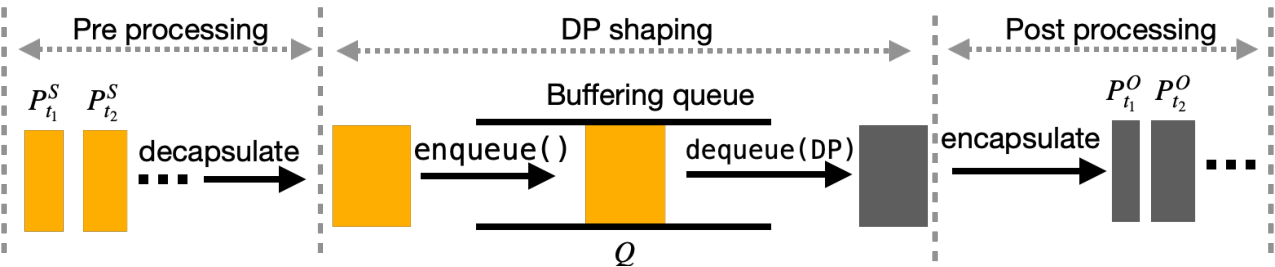
\includegraphics[width=\columnwidth]{figures/DPshaping_concept_vertical.pdf}
    %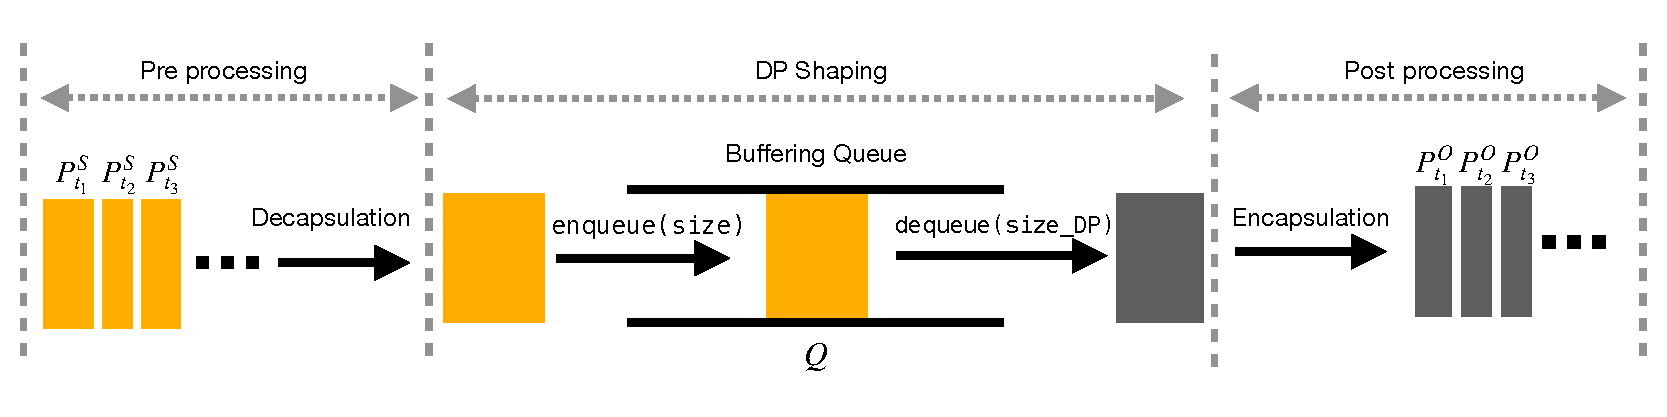
\includegraphics[width=\columnwidth]{figures/DPshaping_concept_horizontal.pdf}
    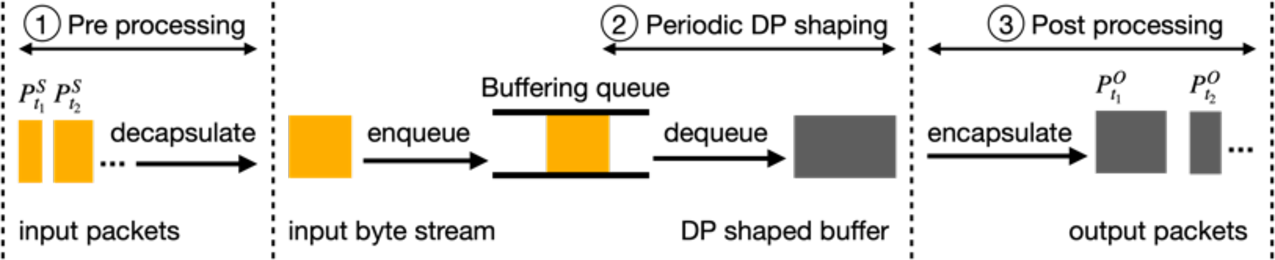
\includegraphics[width=\columnwidth]{figures/dp-overview.pdf}
    \caption{Overview of DP shaping}
    \label{fig:dp-overview}
\end{figure}

%\paragraph{Goal.}
%The design of our traffic shaping algorithm relies on three key steps.
%The rest of this section is organized as follows.
%In \S\ref{subsec:infromation-bottleneck}, we formalize the information available
%to an attacker observing an application stream, which is the sequence of sizes,
%inter-packet intervals, and directions of packets at the finest granularity of
%observation.
%%We propose a primitive of a {\em buffering queue} to collapse all this
%%information into a sufficient statistic to adapt {\sys}'s transmission rate:
%%the
%%size of data in the queue waiting to be transmitted through our shaping
%%mechanism.
%%
%In \S\ref{subsec:dp-queue-measurements}, we describe our decision mechanism for
%sending data based on DP decisions.
%%We show how to perform {\em DP measurements} of our buffering queue, in
%%order to adapt \sys's transmission rate with DP guarantees.
%%We show that under natural constraints on the transmission rate decision
%%mechanism, the change of queue size is bounded, allowing us to perform DP
%%measurements.
%%(\Cref{alg:dp_shaping_mechanism}).
%%Intuitively, we can use DP queue measurements and public information such as
%%network conditions to decide the amount of data to transmit.
%%Transmissions contain queued data when some is available, and dummy data
%%otherwise.
%%The stream observed by any attacker is a post-processing of the DP queries
%%issued on the queue (depends on the private data only through the DP
%%measurements), and is hence DP.
%%
%Finally, in \S\ref{subsec:dp-proof}, we provide a proof sketch for the DP
%guarantees of our shaping mechanism.

%{\as{I don't think we should summarize the intro of DP section into only one
%paragraph. We should give a summary of section here, explaining why we think DP
%shaping is a good idea and how it works Intuitively. More importantly, I think
%we need to  }}
%Specifically, given an application with a corpus of objects, the DP shaping
%ensures that each pair~of {\em neighbouring} objects---whose sizes are within a
%bounded distance---is indistinguishable under DP notion from the observations of
%their traffic shape.
%We denote the maximum distance between any pair of application objects by
%$\ssens$.
%
%Intuitively, {$\sys$} aims to ensure that a stream $S$ is indistinguishable (in
%the DP sense) from a neighboring stream $S'$ by observing the shaped traffic.


\subsection{The Shaping Mechanism}
\label{subsec:infromation-bottleneck}

\Cref{fig:dp-overview} illustrates {\sys}'s $(\epsilon,\delta)$-DP
shaping strategy.
%We denote an application's input packet sequence by
An application's input stream is a packet sequence
$\istream = \{{P^S_1}, {P^S_2}, {P^S_3}, \dots \}$,
%{\as{why do we need a superscript here? it is already defined as $S$.}}
where ${P_i}^S = (l^S_i, t^S_i)$ indicates that the $i$\textsuperscript{th} input
packet in $S$ has length $l^S_i$ bytes and is transmitted at timestamp $t^S_i$.
\ml{We call the total duration of the stream is $\streamduration^S \triangleq
\max t^S_i$.}
Without shaping, an adversary can precisely observe $\istream$ and infer
the content,
% which is any content that is correlated with this stream.
which is correlated with the~stream~\cite{schuster2017beautyburst}.

To prevent this leakage, \sys's DP shaping involves three steps visible on
\Cref{fig:dp-overview}.
%First, the preprocessing step transforms an input stream $S$ over a window
%$\window$ into a byte stream, which is
%accumulated in a {\em buffering queue} $\unshapedQ$. (We denote the length of
%$\unshapedQ$ by $\qlen$.) Specifically, as application packets arrive, {\sys}
%extracts the payload bytes and enqueues them into $\unshapedQ$.
\circled{1} As application stream packets $\istream$ arrive, the preprocessing
step extracts the payload bytes and enqueues them into the buffering queue $\buffQ$.
\circled{2} At periodic intervals $T$, the core DP shaping algorithm
performs a DP measurement $\qlendpt{T}$ of the size of $\buffQ$, to adapt the
amount of traffic send.
The shaping logic then encrypts and enqueues $\qlendpt{T}$ bytes from the
buffering queue $\buffQ$ into the {\em shaped buffer}, using application bytes
available in the queue and dummy bytes if required.
\circled{3} Finally, data in the shaped buffer is split into one or more packets
and transmitted to the network. Since these packets are a post-processing of the
DP-shaped buffer, they preserve DP as long as no new dependency on private data
is introduced.
% This last constraint requires the packets' size and transmit time to be selected
% independently of the data.  We describe how {\sys} enforces this constraint in
% \S\ref{sec:implementation}.

To provide DP guarantees, \sys's shaping relies on two key ideas.
First, it models and controls sensitivity for (potentially long) traffic streams
in over shorter windows of length $\winlen$ \S\ref{subsec:sensitivity}.
Second, it uses its {\em buffering queue} primitive to adapt the transmission
rate to private data $\istream$ while controlling the amount of information
accessible to an adversary \S\ref{subsec:dp-queue-measurements}.
This design enables a rigorous DP analysis of {\sys} \S\ref{subsec:dp-proof}.

% \subsection{The Building Blocks}
% \label{subsec:infromation-bottleneck}

% \Cref{fig:dp-overview} illustrates {\sys}'s $(\epsilon,\delta)$-DP
% shaping strategy.
% %We denote an application's input packet sequence by
% An application's input stream is a packet sequence
% $\istream = \{{P^S_1}, {P^S_2}, {P^S_3}, \dots \}$,
% %{\as{why do we need a superscript here? it is already defined as $S$.}}
% where ${P_i}^S = (l^S_i, t^S_i)$ indicates that the $i$\textsuperscript{th} input
% packet in $S$ has length $l_i$ bytes and is transmitted at timestamp $t_i$.
% Without shaping, an adversary can precisely observe $\istream$ and infer
% the content,
% % which is any content that is correlated with this stream.
% which is correlated with the~stream~\cite{schuster2017beautyburst}.


\subsection{The Sensitivity for DP Measurements}
\label{subsec:sensitivity}

Our DP shaping relies on two key ideas.
%\mis{We actually said in Section 2 that we rely on 3 key ideas.}
First,~it models the DP guarantees for the (potentially long) traffic streams in
windows of fixed length $\winlen$, denoted by \mbox{($\varepsilon_{\winlen},
\delta_{\winlen}$)-DP}.
% An input sequence over $j$\textsuperscript{th} window $j$ is a finite
An input sequence over window $j$ is a finite~sub\-sequence $S_{j} \subset S$,
such that
$S_{j} = \{ P^S_i~|~P^S_i \in S~and~t_i \in j \}$.
{\sys}'s DP guarantees \todo{cover} all (overlapping) windows up to size
$\winlen$.
% \ml{tried to add some hint on how this'll be used to it doesn't sound too weak.}
%$\forall P^S_i \in S_{w_j}, t_i \in w_j$.

% \ml{I moved this here as it's about W and the DP guarantee, it was lower before
% which made it a bit disconnected. I also formalized it a bit more (and
% clarified---I hope---the intuition), this is a key assumption we need to
% reference in the proof later.}
A key assumption for {\sys}'s DP guarantees to hold over $\winlen$-sized windows
\todo{is that the tunnel can always transmit all incoming data from
application streams within any $\winlen$-sized time window.}
In other words, we assume:
%is that the tunnel can handle all incoming data from application streams within
%$\winlen$-sized window of time.
%Specifically, we make the following assumption:
\begin{assumption}\label{assumption:window}
  All bytes enqueued \todo{prior to or} at time $t$ are transmitted by time
  $t+W$.
\end{assumption}
We explain how to realize this assumption in a tunnel design in
\S\ref{sec:design}.
Under this assumption, the privacy loss of the complete traffic stream is
simply a DP composition of the privacy losses over consecutive windows.

The window length $\winlen$ is a configuration parameter, which is set before
the start of an application's transmission. In practice,
%reasonable values for
$\winlen$ would be in the order of a few seconds.
% \ml{[what does that part of the sentence mean? We do sliding windows for the
% guarantee, not consecutive windows, so I don't think we need alignment? I
% suggest removing that part:] and the windows could be aligned with the
% boundaries of a packet sequence in one direction}.

Secondly, we use the primitive of a {\em buffering queue} to control the
maximum information accessible by an adversary within each window. We denote the
number of bytes present in the queue (\ie length of the queue) by $\qlen$.
%The buffering queue has three operations: {\em enqueue}, {\em dequeue}, {\em
%get\_size}.
Conceptually, {\sys} extracts bytes from the input stream, $\istream$, and
enqueues them.
%At the beginning of each window, {\sys} retrieves the queue length and
%determines the amount of data to dequeue to transmit it as shaped
%traffic.
{Further, we discretize time into $\winlen$-sized windows and, at the
beginning of each time window, {\sys} adds a DP noise to the queue
length to determine the amount of data from the queue that should be transmitted
as shaped traffic.}
The shaped traffic is then transmitted as a packet sequence denoted by $\ostream
= \{{P^O_1}, {P^O_2}, {P^O_3} \dots \}$, which is observable by an adversary.
{While shaping requires discretizing transmit windows, the DP guarantees
apply over arbitrary windows.}
%The DP shaping transforms $\istream$ to $\ostream$, where the packet sizes and
%timings are derived from distributions such that they provide DP privacy
%guarantees.

% %As indicated in \S\ref{subsec:DP-background}, DP guarantees rely on a
% %notion of neighboring datasets and the maximal change in a query result based
% %on a single change in the dataset.
% %Determining DP guarantees on an application's complete traffic streams (which
% %may have arbitrary lengths) would be expensive as the maximal difference to the
% %transmission length would be the difference of the largest and smallest objects
% %in the application's dataset.
% %Since reasoning about infinite streams is impractical {\as{why it is
% %impractical?}},
% A key assumption for {\sys}'s DP guarantees over $\winlen$-sized windows is that
% the tunnel can handle consecutive windows of transmission on application streams
% independently, \ie all bytes present in the buffering queue at the beginning of
% the $j$\textsuperscript{th} window are transmitted within $j$
% before the application transmits bytes in the $(j+1)$\textsuperscript{th}
% window. (We explain how to realize this assumption in a tunnel design in
% \S\ref{sec:design}.)
% Under this assumption, the privacy loss of the complete traffic stream \todo{is
% simply a sum of the privacy losses} over consecutive windows.
% %\am{Verify correctness.}\as{I think it should be rephrased with "under this
% %assumption, the privacy loss of whole traffic trace is simply composition of
% %privacy loss of consecutive windows." Note that summation of privacy loss is a
% %basic form of composition (it gives the resutls that is larger than actual
% %privacy loss), and we always can use either advanced composition or other
% %methods such as Renyi-DP to calculate privacy loss more accurately.}
% %{\as{the privacy loss always grows with number of windows. The assumption helps
% %us to pick up small numbers for sensitivity, and as a result, add less noise. If
% %we assume data can accumulate in queues (i.e. have large $W$), the value for
% %$\Delta^W$ became larger and so the value of $\Delta^T$ and as a result, the
% %noise value.}}

In the rest of this section, we focus on {\sys}'s DP guarantees over a single
window.
We first formally define a notion of ($\varepsilon_\winlen$,$\delta_\winlen$)-DP
privacy, which guarantees DP over transmission windows of length $\winlen$.
The guarantee applies over all $\winlen$ windows, and applying DP
composition yields guarantees over multiple windows.
Then, we provide an overview of the DP shaping mechanism, which further samples
noise in multiple shorter uniform intervals within each window.
Finally, we prove how the shaping mechanism provides
($\varepsilon_\winlen$,$\delta_\winlen$)-DP.
%\am{Do we prove or define?}

To formalize {\sys}'s DP guarantees, we first define a meaningful
distance between any pair of streams in windows of length $\winlen$ and the
associated neighboring definition:

%Application's traffic streams may have arbitrary lengths.
%Thus, instead of computing DP guarantees over entire streams, {\sys} reasons
%about DP guarantees in windows of fixed length $\winlen$.

\begin{definition}
Two streams $S_{j}$ and $S_{j}'$ transmitted in a window $j$
are neighbors
%    if, within each time window $\window$,
if their L1-norm distance is at most~$\ssens$ bytes in
\todo{a window of upto length $\winlen$}, \ie
%any window, \ie
${\norm{~S_{j} - S_{j}'~}}_1 \leq \ssens$.
%    in any time window of size $\window$:

%\begin{equation}\label{equ:stream-neighboring}
%%    \sum_{t \in \window} {\norm{S_t - S'_t}}_{L_1} \leq \ssens \; (bytes)
%{\norm{S - S'}}_{L_1} \leq \ssens \; (bytes)
%\end{equation}
\label{def:neighboring-streams}
\end{definition}

$\ssens$ is the max L1-norm distance between each pair of application streams
transmitted in any window $j$.
We utilize the L1-norm (the sum of absolute values) as our distance metric
to quantify the dissimilarity between two traffic streams, as it captures
differences in both packet sizes and \todo{temporal pattern.}
%timing.
% \am{Do we need to expand the L1-norm definition?}
% \as{I think it adds more complexity. we can skip that.}
%Here, $\norm{S - S'}}_{L_1} = \sum_{t \in \window} | |$
%We utilize the L1-norm as our distance metric to quantify the dissimilarity
%between two traffic streams, as it captures differences in both segment size and
%temporal pattern.

%The DP guarantees require a key assumption that $\ssens$ is bounded and that
%{\sys} can transmit all payload bytes of the streams within $w$.
%(We explain how to realize this assumption in a tunnel design in
%\S\ref{sec:design}.)
%Under this assumption, consecutive windows of transmission streams have the
%same ($\epsilon_w$,$\delta_w$)-DP privacy guarantees.


%\paragraph{Key idea.}
%To implement DP shaping, {\sys} relies on a primitive of {\em buffering queue}
%$\unshapedQ$, which accumulates the payload bytes from an application stream,
%before they are packaged into DP-sized bursts.
%The DP guarantees rely on a key assumption that all payload bytes accumulated
%in $\unshapedQ$ within a window can be transmitted within the window.
%At the beginning of each
%interval, the DP shaping logic computes a DP burst size based on noise sampled
%from a DP distribution and the total number of bytes available in $\unshapedQ$.
%Applying DP in intervals and over an abstract queue independent of the
%application streams obviates the need for profiling complete application
%streams and enables dynamic adaptation during shaping.

\ml{Add discussion about an upper bound here, and say we can also use something smaller.}

% \subsection{The Shaping Mechanism}
\subsection{Adaptive Shaping with DP Measurements}
\label{subsec:dp-queue-measurements}

\paragraph{From windows to intervals.}
%\am{Add rationale for moving from $\winlen$ to $\dpintvl$.}
{Based on \Cref{assumption:window} and \Cref{def:neighboring-streams},}
the window length $\winlen$ affects the maximum number of bytes that can be
accumulated in the buffering queue (thus, the maximum distance between stream
pairs), as well as the transmission delay for the payload bytes enqueued.
Specifically, large windows lead to high-latency bursty traffic.
\shepherd{To reduce latency and burstiness}\as{comment 1.b: we should explain how does having two windows recduce the burstiness and why we cannot make W as small as T}, {\sys} further splits windows into
smaller intervals of length $\dpintvl$ and samples noise at the beginning of
each interval.
\todo{In absence of shaping, the queue length corresponds to the amount of
    unshaped traffic transmitted in an interval of $\dpintvl$.}
The privacy loss over a window is now defined by applying DP composition
on the privacy loss of individual intervals.
%\am{We need to discuss in the evaluation how the total privacy loss (and
%overhead) using DP composition over N intervals compares with the privacy loss
%due to a single DP interval of the same length as the window length.}
%\as{I think we are already doing that. The plot that shows different amount of
%privacy loss for different number of updates is there. The missing factor is,
%however, the overheads (both bandwidth and latencies). The less we measure the
%queue size and adapt the shape of traffic to it, more overhead we add. In the
%extreme scenario, if we measure only once, it is exactly like constant rate
%shaping where the rate is decided at the measurement time.}
%performs real-time, dynamic traffic shaping on a continuous stream of traffic.
%To do this, as shown in \Cref{fig:dp-overview}, we rely on a primitive of a
%{\em buffering
%queue} to implement shaping.
%%The queue is used to accumulate the payload bytes from an application's packet
%%sequence $S_{\winlen}$ and subsequently to transmit the bytes into DP-sized
%%bursts.
%%{\as{this is the first time we talk about DP-sized bursts
%        %and it might be confusing for the reader.}}
%We denote the number of bytes
%present in the queue (\ie length of the queue) by $\qlen$. {\sys}
%samples noise at periodic intervals of length $\dpintvl \leq \winlen$.

To apply noise in each interval, we now define the sensitivity of
the queue length over intervals of length $\dpintvl$.
Sensitivity, denoted $\qsens$, is the maximum difference in the queue length
over any interval $\dpintvl$ that can be caused by changing one application
stream to another.
% over any interval of length $\dpintvl$ due to any pair of different application
% streams.
%We define $\qsens$ as the sensitivity of the variable $\qlen$, which is the
%maximum change in $\qlen$ over an interval of length $\dpintvl$ when the
%application stream passing through the buffering queue changes from one to
%another.
%Suppose, the state of the buffering queue is $\unshapedQ$ and $\unshapedQ'$
%at the start of the transmission of stream $\streamw{j}$ and $\streamw{j}'$,
%respectively.
Formally, consider two alternative streams $\streamw{j}$ and
$\streamw{j}'$ passing through the queue.
Suppose that when transmitting $\streamw{j}$ (similarly $\streamw{j}'$), the
queue length at the beginning of its $k$\textsuperscript{th}
interval is denoted by $\qlent{k}$ (respectively $\qlent{k}'$).
%Similarly, when transmitting $\streamw{j}'$, the queue length at the beginning
%of its $k$\textsuperscript{th} interval is denoted by $\qlent{k}'$.
%Furthermore, suppose the length of $\unshapedQ$ and $\unshapedQ'$ at the
%beginning of an interval $\tau$ is denoted by $\qlent{\tau}$ and
%$\qlent{\tau}'$, respectively.
Then:
\setlength{\abovedisplayskip}{0pt}
\begin{equation}
    \qsens = \max_{k = 0}^{\numupdates}~\max_{\streamw{j},
        \streamw{j}'} | \qlent{k} - \qlent{k}' |
    \label{eqn:ssens}
\end{equation}
%
%\am{I find it weird that we have independent windows but shorter intervals
%within windows for which we apply DP composition. To make things even more
%confusing, we will have another interval in the implementation for simply
%prioritizing payload bytes over dummy. We need to explain all the different
%intervals very clearly.}
%\as{Maybe we need to discuss it with others in group.}

%\smallskip\noindent
\paragraph{Shaping overview.}
\sys's DP shaping involves three steps as shown in \Cref{fig:dp-overview}.
%First, the preprocessing step transforms an input stream $S$ over a window
%$\window$ into a byte stream, which is
%accumulated in a {\em buffering queue} $\unshapedQ$. (We denote the length of
%$\unshapedQ$ by $\qlen$.) Specifically, as application packets arrive, {\sys}
%extracts the payload bytes and enqueues them into $\unshapedQ$.
\circled{1} As application packets arrive in a window $\window$, the
preprocessing
step extracts the payload bytes and enqueues them into the buffering queue.
\circled{2} In a periodic interval $k$, the core DP shaping algorithm
{performs a DP measurement, which entails} sampling noise $z$ from a DP
distribution and computing a DP burst size
$\qlendpt{k} \triangleq \qlent{k} + z$.
%based on the sampled noise and the total number of application bytes
%available in the buffering queue,
The shaping logic then
prepares a {\em shaped buffer} of length $\qlendpt{k}$ with
the application bytes available in the queue and dummy bytes if required.
The DP shaping logic uses an additive Gaussian noise mechanism.
The noise $z$ is sampled from a normal distribution
$\mathcal{N}\big(\mu,~\sigma^2\big)$ parameterized by $\epsilon_\dpintvl$,
$\delta_\dpintvl$, and~$\qsens$:
%\mbox{$\mathcal{N}\big(\mu = 0,~\sigma^2 =
    %\frac{2\Delta}{\varepsilon}\ln(\frac{1.25}{\delta})\big)$}.
The mean $\mu$ is 0 and the variance $\sigma^2$ is given by
%$(2\qsens/\varepsilon)\ln(1.25/\delta)$.
$\frac{2\qsens^2}{\varepsilon_\dpintvl^2}\ln(\frac{1.25}{\delta_\dpintvl})$.
{If the sampled noise is negative, we retain some of the data in the
queue until the next DP measurement interval.}
Given this noise distribution, one measurement is \mbox{$(\epsilon_\dpintvl,
\delta_\dpintvl)$-DP}.
%\am{What is the explanation of 1.25?}{\as{it is a constant factor as part of
%Gaussian additive noise mechanism}}
%
\circled{3}~Data in the shaped buffer is then split into one or more packets
and transmitted to the network. Since these packets are a post-processing of the
DP-shaped buffer, they preserve DP as long as no new dependency on private data
is introduced. This last constraint requires the packets' size and transmit time
to be selected independently of the data.
We describe how {\sys} enforces this constraint in \S\ref{sec:implementation}.

%{\bf D1.} We formalize the information available to an adversary observing an
%application's traffic, which includes packet sizes and the precise timing at
%which each packet is transmitted from an application.
%{\bf D2.} We define a primitive of a {\em buffering queue} which accumulates the
%payload bytes extracted from an application's packet sequence and from which
%bytes are used to prepare a DP sized buffer from transmission.
%\todo{Indeed, we show that under natural constraints on the transmission rate
    %decision mechanism, the change of queue size is bounded, allowing us to
    %perform
    %DP measurements (\S\ref{subsec:dp-queue-measurements}).}
%{\bf D3.} We discuss the core DP shaping logic, which involves periodically
%sampling noise from a DP distribution, computing a DP burst size based on the
%sampled noise and the total number of payload bytes available in the buffering
%queue, and preparing a buffer with payload and (optional) dummy bytes of length
%equal to the computed DP burst size.
%\todo{Intuitively, we can use DP queue measurements and public information such
%as network conditions to decide the amount of data to transmit.
%The stream observed by any attacker is a post-processing of the DP queries
%issued on the queue (depends on the private data only through the DP
%measurements), and is hence DP.}

%We elaborate on the details now. We start with a formal definition of
%neighboring streams and the sensitivity ($\ssens$) of a variable denoting the
%distance between any pair of streams.

%\paragraph{Assumption.}
%The DP guarantees of the shaping mechanism rely on a key assumption: the
%length $\qlen$ in any interval $\window$ has a fixed upper
%bound. This bound, denoted by $\qsens$, corresponds to the sensitivity of the
%variable $\qlen$, which is the maximum change in $\qlen$ when the application
%stream passing through $\unshapedQ$ changes from one to another.


%\paragraph{Noise.}
%As mentioned above, at periodic intervals, the DP shaping logic samples noise
%from a DP noise distribution and computes $\qlendp$ by adding the noise to
%$\qlen$. The DP shaping logic uses an additive Gaussian noise mechanism.
%Mathematically, we denote the length of $\unshapedQ$ at the beginning
%of an interval $\tau$ by $\qlent{\tau}$ and the burst length resulting from
%adding noise $z$ to it as
%$\qlent{\tau}^{\epsilon, \delta} \triangleq \qlent{\tau} + z$.
%The noise $z$ is sampled from a normal distribution
%$\mathcal{N}\big(\mu,~\sigma^2\big)$ parameterized by $\epsilon$,
%$\delta$, and~$\qsens$:
%%\mbox{$\mathcal{N}\big(\mu = 0,~\sigma^2 =
%%\frac{2\Delta}{\varepsilon}\ln(\frac{1.25}{\delta})\big)$}.
%The mean $\mu$ is 0 and the variance $\sigma^2$ is given by
%%$(2\qsens/\varepsilon)\ln(1.25/\delta)$.
%$\frac{2\qsens}{\varepsilon}\ln(\frac{1.25}{\delta})$.

%The privacy guarantees and the bandwidth overheads of the DP shaping depend on
%five parameters:
%$\qsens$, $\epsilon_\dpintvl$, $\delta_\dpintvl$,
The privacy loss ($\varepsilon_{\winlen}$) and bandwidth overheads of the DP
shaping (represented by $\sigma_\dpintvl$, \ie the standard deviation of the
noise distribution function) depend on
$\winlen$, $\ssens$,
%$\varepsilon_{\dpintvl}$, $\delta_{\dpintvl}$,
and the number of intervals $\varnumupdates = \numupdates$ in $\winlen$.
Additionally, the latency overheads depend on $\dpintvl$.
Note that for a specific value of $\ssens$ and $\varnumupdates$, the DP guarantee
$\varepsilon_{\winlen}$ is fully specified by $\sigma_\dpintvl$, and remains the same even at
different time scales.
That is, scaling $\winlen$ and $\dpintvl$ proportionally does not change the
privacy and overhead costs.
%{\as{We are not sure about this, the latency can be affected by the amount of
%noise in extreme scenarios}}
We analyze the impact of different choices for these parameters on
the privacy guarantees and overheads in \S\ref{sec:eval}. Here, we focus on a
formal model of the DP guarantees.

%Our differentially private traffic shaping strategy ensures that the attacker
%is not able trace back any traffic pattern transmitted over a public network to
%its original pattern. This is achieved by shaping the traffic stream such that
%any neighboring set of traffic streams has an equal probability of producing the
%observed pattern. We will elaborate on our definition of neighboring streams in
%the next section.

%A key feature of $\sys$'s design is to ensure that the amount of data in a queue
%can only change by at most $D_s$ when changing a stream $S$ by a neighboring
%$S'$. We elaborate on this in \Cref{sec:design}.

\subsection{Privacy Guarantees}
\label{subsec:dp-proof}
%\as{I think we need to change the title of this section as it is not the proof
%but also proposing our guarantees. I suggest the title: "Privacy guarantees".}
At a high level, analyzing the  ($\varepsilon_{\winlen}, \delta_{\winlen}$)-DP
guarantee of the overall shaping mechanism requires two steps: (i) showing that
the difference in the buffering queue length is bounded for neighboring streams
for all transmissions of the streams (Prop. \ref{prop:sensitivity}), and (ii)
composing the DP cost of each measurement over the intervals defining a window
of length $\winlen$ (Prop. \ref{prop:dp}).
%\todo{(i) two neighboring streams in windows of length $\winlen$ are neighbors
%during all transmit intervals of length $\dpintvl$, and (ii) the total privacy
%loss composed over all transmit intervals within a window amounts to the privacy
%loss defined over the entire window.}
%\am{Verify wording.}
%\as{I think the wording is wrong for both points. We need to show that
%difference in queue lengths are bounded. Then the second point naturally follows
%by composition.}
%(i) the neighboring definition over the buffering queue length over intervals
%$\dpintvl$ implies neighboring definition

%Formally, {$\sys$} offers the following guarantee:
We first show that the sensitivity of each measurement $\qsens$ is at most the
window sensitivity $\ssens$:
\begin{proposition}\label{prop:sensitivity}
    {$\sys$} enforces $\qsens \leq \ssens$.
\end{proposition}

\begin{proofsketch}
  Consider any two streams $S_j$ and $S_j'$, as in \Cref{eqn:ssens}.
  The proof proceeds in two steps. First, under \Cref{assumption:window},
  streams can accumulate queued traffic for at most {$\winlen$}, so two
  different streams can create a difference $|\qlent{k} - \qlent{k}'|$ of at
  most $\ssens$.
  Second, dequeuing can only make two different queues closer: Consider
  measurement time $k$, with queue lengths $\qlent{k} > \qlent{k}'$ (the
  opposite case is symmetric).
  For a DP noise draw $z$, we have $\qlendpt{k} > \qlendpt{k}'$. Since shaping
  sends at least as much data under $\qlendpt{k}$ as under $\qlendpt{k}'$,
  but no more than $\qlendpt{k} - \qlendpt{k}'$, after dequeuing we have
  $|\qlent{k+1}' - \qlent{k+1}| \leq |\qlent{k}' - \qlent{k}|$.
  In summary, the maximum queue difference under two different streams
  $\qsens$ can grow to at most $\ssens$ due to data queuing, and dequeuing only
  decreases that difference, and hence $\qsens \leq \ssens$.  The complete proof
  is in \S\ref{appendix:dp}.
\end{proofsketch}

We can then reason about DP guarantees over intervals of length $\dpintvl$ in
order to achieve the privacy loss for the entire window of length $\winlen$.
%
Formally, we have:
\begin{proposition}\label{prop:dp}
  {$\sys$} enforces $(\varepsilon_{\winlen}, \delta_{\winlen})$-DP, with
  $\varepsilon_{\winlen}, \delta_{\winlen} \triangleq
  \textrm{DP\_compose}(\varepsilon_T, \delta_T, \numupdates)$.
\end{proposition}

\begin{proof}
By Prop. \ref{prop:sensitivity}, the sensitivity of each measurement is at most
  $\ssens$.
%\am{I thought the sensitivity is already defined in \Cref{eqn:ssens}.}
By the Gaussian DP mechanism, the measured queue size $\qlendpt{k}$ in each
interval $k$ of length $\dpintvl$ is $(\varepsilon_{T}, \delta_{T})$-DP.
% Over a time window of length $\winlen$, {\sys} will sample noise
% $\numupdates$ times.
Using DP composition over $\numupdates$ $(\varepsilon_{T}, \delta_{T})$-DP
measurements, and the fact that $\ostream$ is a post-processing of DP
measurements, yields the ($\varepsilon_{\winlen}, \delta_{\winlen}$)-DP over
any $\winlen$ length window.
% By using R\'enyi algorithm for DP\_compose(), we get $\varepsilon$,
% $\delta$ that correspond to ($\varepsilon_{\winlen}, \delta_{\winlen}$)-DP
% definition over $\winlen$ windows.
%\todo{Thus, the proof concludes with the application of DP composition.}
%\am{I am not sure how the last line follows from the second last line: what does
%it mean say proof concludes with application of DP composition.}
%\as{It is just the way of saying that compositions is applied here and privacy
%parameters, $\varepsilon_W, \delta_W$ are result of it.}
\end{proof}
We use R\'enyi-DP composition on the Gaussian mechanism for
$\textrm{DP\_compose()}$.
%If $\winlen$ is larger than all traffic streams, {$\sys$} enforces
%$(\varepsilon_{\winlen}, \delta_{\winlen})$-DP over all streams going through he
%shaped tunnel. \am{Not sure what the previous statement is trying to
%say.}{\as{I also think maybe it is better to remove it}}
Note that the overhead (\ie noise added) due to
DP does not depend on the number of streams: the overhead is the same regardless
of the number of streams transmitted through the buffering queue simultaneously.


%\smallskip\noindent
\paragraph{Summary.}
By buffering all data in a queue, and periodically deciding the size of the data
to send over the network with a DP measurement, \sys's shaping algorithm
makes the shape of traffic (volume of data sent over time) DP with regards to
the application's original traffic sequence.
%The DP shaping algorithm ensures that an adversary cannot trace the observed
%packet sizes on the network back to the packet sizes in the application's
%original sequence.
% The DP shaping algorithm makes \ml{the amount of traffic \sout{the packet sizes}
% output} on the network independent of (DP with regards to) the amount of traffic
% in the application's original sequence, in each window of size $\winlen$.
% of the packet sizes in the application's
% original sequence.
% \ml{[this is wrong without the later timing things I think, shoule remove? Or at
% least should be refined, I'm not too sure what the goal is here] Furthermore,
% due to the periodic execution of algorithm and the subsequent DP post processing
% property, the timing of output packets is also independent of the packet timings
% in the original sequence.}
Thus, as long as no observable characteristics of the traffic directly depend on
application secrets (the original traffic sequence), the observable outbound traffic
is DP.
% Thus, the algorithm ensures that the shape of the outbound traffic of an
% application is independent of application secrets.

%\am{The proof of the DP guarantees of the algorithm is provided in the
%appendix. Can we prove that constant timing intervals + differentially privacy
%on size = differentially privacy on the overall traffic shape?}

\ml{\paragraph{Interpretation} Let's add something on interpreting the guarantees and what they mean here: hidding any marginal change of size sensitivity (presence + content); composition over time; group composition for larger sensitivity.}

%%%%%%%%%%%
%% old text
%%%%%%%%%%%
% \paragraph{Unshaped queue.}
% We model an abstract queue, {$\unshapedQ$}, which holds the unshaped input byte
% stream of an application and supports two operations: enqueue and dequeue.

% \paragraph{Neighboring queue states.}
% We define the queue state, ${\unshapedQ}_{\tau}$, as the amount of traffic
% inside ${\unshapedQ}$ at time $\tau$. We call two queue states, ${\unshapedQ}_{\tau}$
% and ${\unshapedQ}'_{\tau}$, neighbor queue states if and only if we have:
% \begin{equation}\label{equ:queue-neighboring}
        % |{\unshapedQ}_{\tau} - {\unshapedQ}'_{\tau}| \leq D_q \;(bytes)
% \end{equation}
% where $D_q$ is a parameter in our system.


% \paragraph{Query function and sensitivity.}
% We define a query function on the queue state ${\unshapedQ}$,
% $f({\unshapedQ}_{\tau})$, as a function that returns the
% size of the queue at time ${\tau}$. The sensitivity of the function $f$ is given~by:
% \begin{equation}
% \Delta_1 f = \max_{Q, Q'} \| f(Q_{\tau}) - f(Q'_{\tau}) \|_1 =  \max_{Q, Q'} \| Q - Q' \|_1 = D_q
% \end{equation}
% Here, $\Delta_1 f$ captures the magnitude by which the size of queue can change
% from one stream to another.  In fact, {\sys}'s shaping strategy guarantees that
% the queue size cannot be accurately ascertained by an attacker.  At this point,
% we have all necessary building blocks to propose our differentially private
% shaping algorithm.

% \paragraph{From queues to traffic streams.}

% The definition presented in \Cref{equ:queue-neighboring} serves as a sufficient
% basis for designing our differentially private traffic shaping based on queue
% states.  However, in order to provide comprehensive privacy guarantees for
% internet applications, we extend this definition from queue states to
% streams of traffic.


% To reason about the privacy of traffic streams, we need to define neighboring
% streams (i.e. the minimal protection unit of each differentially private
% algorithm).  Two stream prefixes, $S_t$ and $S'_t$ (with the representation of
% \Cref{equ:stream-segs}), are neighbors if and only if:
% \begin{equation}\label{equ:stream-neighboring}
        % \|S_t - S'_t\|_1 \leq D_s \; (bytes)
% \end{equation}
% We utilize the L1-norm as our distance metric to quantify the dissimilarity
% between two traffic streams, as it captures differences in both
% segment size and temporal pattern.


% Our goal is to measure, and subsequently bound, the privacy loss of a traffic
% stream.
% Intuitively, an attacker's observation of a traffic stream can be interpreted as
% a series of differentially private queries on the segment sizes of original
% traffic pattern. \am{I find this intuition of an attacker issuing DP queries
% strange. To me, the attacker performs usual queries on a database whose
% underlying distribution has been made DP.}
% We claim that the privacy loss for a individual traffic stream shaped with our
% mechanism can be quantified by aggregating the privacy loss incurred at each
% measurement of the abstract queue size.
% The following statement provides a formal representation of this notion.


% \ml{Amir, please use real latex things for the Claim and Lemma. I'd also call the Lemma Proposition instead: Lemma is for general theoretical tools others might reuse and apply to other proofs).}
% \textbf{Claim}: The privacy loss of transmitting a traffic stream with the
% length of $w = kT$ through the {\sys} middle-box, is the composition of $k$
% queries on the queue state.
% \\
% To show that this claim is true, we only need to prove the following lemma.

% \textbf{Lemma}: Assume two neighboring traffic streams, $S_t$ and $S_t'$,
% transmitted through a middle-box with \Cref{alg:middle-box-all} as the shaping
% mechanism. If they both reshaped to the same traffic stream, $S_O$, then,  at
% any given time $\tau$, the queue states for neighboring streams are $D$-close.
% In other words we have:
% \begin{equation}\label{equ:composition_dp_section}
        % \forall \tau > 0 : |Q_{\tau} - Q_{\tau}'| \leq D
% \end{equation}
% where $D = \min(D_q, Q_{max})$. $D_q$ and $Q_{max}$ are the queue neighboring
% threshold and maximum buffer size of our middle box respectively.
% \am{I see no relation between $D_q$ and $D_s$.}

% This means the unshaped queues of these two streams are always neighbors
% according to the neighboring definition of \Cref{equ:queue-neighboring}.
% We prove the Lemma in \Cref{appendix:dp}.

% Here, we show how we can calculate privacy loss for a traffic stream.
% Assume two neighbor streams, $S_t$ and $S_t'$, reshaped to the same stream,
% $S_O$, by {\sys} middle-box. If we show the shaping mechanism by $M_s$, the
% privacy loss is:
% \begin{equation}\label{equ:privacy-loss}
  % \log\big(\frac{\Pr[M_s(S_t)=S_O]}{\Pr[M_s(S_t')=S_O]}\big) \leq \varepsilon_g
% \end{equation}
% Using the representation of \Cref{equ:stream-segs}, we have:

% \todo{Add the equation}

% The composition comes into the picture in the inequality \todo{Add ref} as the
% size of output at each round depends on the amount traffic enqueued into the
% ${\unshapedQ}$ and outputs of previous rounds of the mechanism, which both
% abstracted in the queue state.

\if 0
\subsection{DP shaping building blocks}
\label{subsec:infromation-bottleneck}
We define a source application stream $S$ as a sequence of packets
$\{P_{t_1}^{l_1}, P_{t_2}^{l_2}, P_{t_3}^{l_3}, \dots \}^S$
%$\{P_{t_1}^{l_1}, P_{t_2}^{l_2}, P_{t_3}^{l_3}, \dots \}^S = \langle(l_1, t_1),
%(l_2, t_2), (l_3, t_3), \dots \rangle^S$,
where $l_i$ and $t_i$ respectively indicate the length in bytes and timestamp of
the $i$\textsuperscript{th} packet of the stream $S$.
%\begin{equation}\label{equ:stream-pkts}
%        $S = \{P_{t_1}^S, P_{t_2}^S, P_{t_3}^S, \dots \}$,
%\end{equation}
%where $P_{t_i}^S$ is the size of the packet transmitted as a part of the stream
%$S$ at the time $t_i$.
%
Without shaping, an adversary can observe this precise stream and infer
the content, which is correlated with this stream.

In {\sys}, we first introduce an information bottleneck in the form of a
buffering queue, {$\unshapedQ$}, to control the information accessible by an
eavesdropper. The buffering queue has three operations: \texttt{enqueue(size)},
\texttt{dequeue(size)}, \texttt{get\_size()}.
Conceptually, {\sys} decapsulates all application traffic of incoming stream
$S$, and enqueues it in the {$\unshapedQ$}.
The shaping mechanism in {\sys} periodically retrieves the queue size and
determines the amount of data to dequeue from $\unshapedQ$ in order to transmit
it as shaped traffic.
The shaped traffic is encapsulated into a new sequence of packets, which we
denote as:
\begin{equation}\label{equ:stream-segs}
    O = \{P_{t_1}^O, P_{t_2}^O, P_{t_3}^O, \dots\}
\end{equation}
where $P_{t_i}^O$ is a packet sent in the shaped tunnel.

In order to ensure that the observable stream $O$ preserves the privacy of the
original stream $S$, {\sys} ensures that $O$ is Differentially Private.
To enforce DP, {\sys} ensures that any input to $O$ that depends on sensitive
data (the stream $S$) is measured with DP.
\Cref{fig:dp-overview} shows the end-to-end traffic shaping of {\sys}.
After decapsulating incoming packets, the incoming traffic is stored in a
buffering queue. In fixed periods, the \texttt{dequeue} operation is performed,
ensuring that the timing of the outgoing traffic remains independent of the
incoming traffic. The size of the \texttt{dequeue} is determined by our
differential privacy mechanism, guaranteeing that the size of the outgoing
traffic remains DP.
Furthermore, the encapsulation and packetization of outgoing data can be
characterized as a post-processing step of a differentially private mechanism
and therefore is DP.
\fi


\if 0
\subsection{DP shaping mechanism}
\label{subsec:dp-shaping}

\ml{I feel like this all belong to \am{design} with the DP call as a noisy black
box.} \am{Yes, this is covered in \S\ref{subsec:design-overview}.}

\Cref{alg:middle-box-all} represents the differentially private shaping
mechanism.  The algorithm is executed periodically with an interval of $T$
seconds.  Here, we explain one round of the algorithm.
\begin{enumerate}
  \item The DP mechanism reads the current size of the queue, $Q_t$.
  \item Then, it adds a noise from a Gaussian distribution with an average of
  zero and scale of ${\sigma}$ to the current size. The noisy measurement is
  represented by $D^S_t$ in the algorithm, and $\sigma$ is the parameter that
  determines the privacy loss of our mechanism.
  \item To avoid unpredictable behaviors such as the occurrence of negative
  values in the noisy measurement, we have incorporated a minimum and maximum
  size threshold for the noisy measurements, which are adjustable parameters
  within the algorithm.
  \item If $D^S_t > Q_t$, the data in {\unshapedQ} will be padded to $D^S_t$
  bytes and subsequently transmitted to the receiver.
  Conversely, if the size of the data in {\unshapedQ} is less than or equal to
  $D^S_t$, the entirety of the $D^S_t$ bytes will be sent.  In algorithm
  \ref{alg:middle-box-all}, the padding size and real data size are represented
  with $D^P_t$ and $D^R_t$ respectively.
\end{enumerate}
\fi

